\documentclass[a4paper, 11pt, titlepage]{article}
% \usepackage{geometry}
% \usepackage{longtable}
\usepackage{tabularx}
\usepackage{setspace}
\usepackage[backend=biber]{biblatex}
\usepackage{bm}
\usepackage{amsmath}
\usepackage{hyperref}
\usepackage{graphicx,float}
\usepackage[export]{adjustbox}

% \nocite{*}

% \newcommand{\vmiddle}[1]{\begin{tabular}{l} #1 \end{tabular}}
% \renewcommand\tabularxcolumn[1]{m{#1}}% for vertical centering text in X
% column



\title{COMP5900C\\
Assignment 1\\
Low-Level Texture Synthesis}
\author{Gabriel Racz}

\begin{document}
\maketitle
\section{Target}
The goal of this report is to synthesize a texture similar to the following\\\\
\adjustbox{center} {
    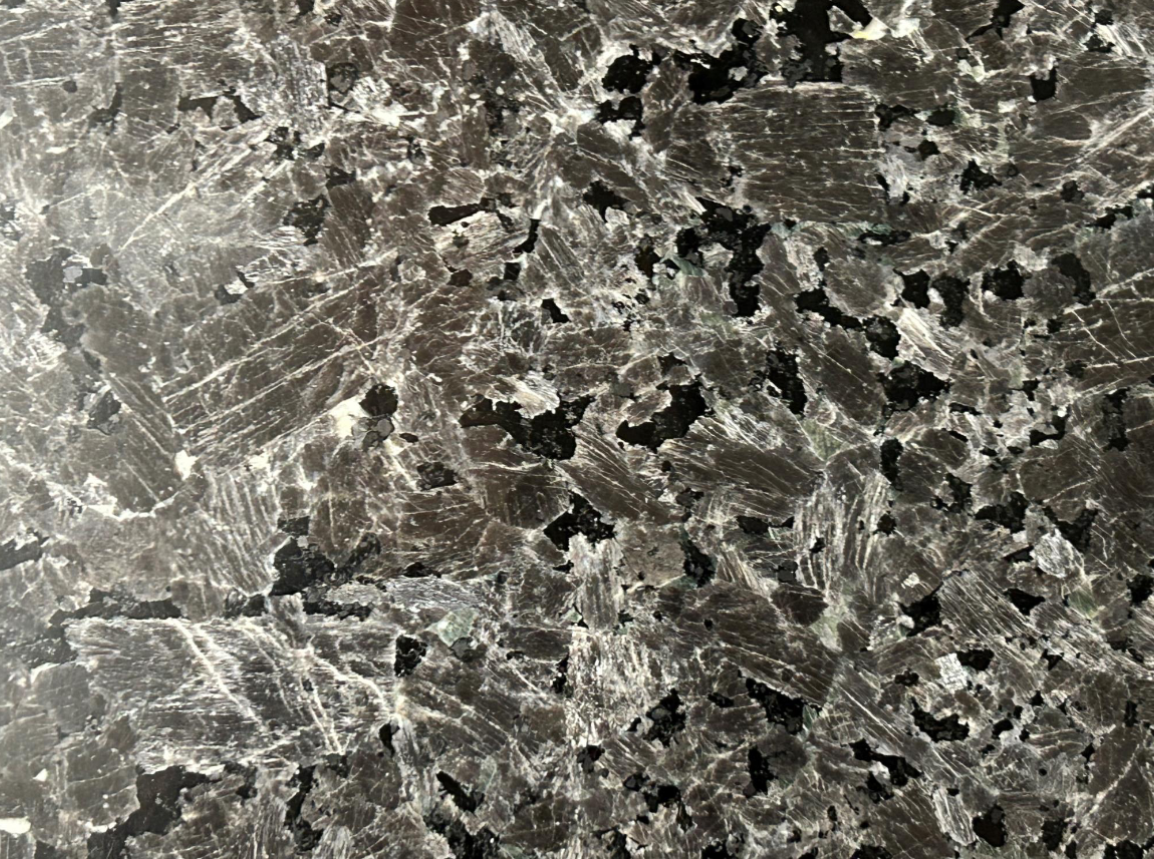
\includegraphics[width=4.0in]{images/sample.png}
}
using low-level image processing operations in combination with parametric noise.
This granite-like texture is particularly interesting from a pure structural
synthesis point of view at it has depends very little on color and relies on
strong contrast and clear sharp lines to define both high and low frequency
features.

The synthesis approach described was inspired by both the properties of real-world granite
counter top materials and the natural intuition to segment textures into
repeating or layered shapes. The texture generation procedure is based on
generating granite ``shards'' at various scales and layering to create the
illusion of depth. 

The silhouette of a single granite shard is composed of a more or less convex
polygon with jagged edges, textured with various frequencies of straight bright
cracks that are generally anisotropic over a single shard. At this resolution,
the background beneath the shards seems to be composed of a dark and relatively
continuous noise with small specular pieces embedded within it.

Therefore, the high-level strategy followed for creating similar textures was:
\begin{enumerate}
    \item Generate shard shapes
    \item Texture shard interiors
    \item Layer shards overtop one another
    \item Fill empty regions with background
\end{enumerate}
\section{Approach}
\subsection{Shard Generation}
To generate the shards, I knew that a thresholded noise function generally
created isolated splats that reliably appeared as random polygon silhouettes.
As the noise basis for this implementation, simplex noise was used to an
\href{https://gist.github.com/kibotu/1cad8664c8b181cdc4e2}{excellent open source
implementation} being available for Processing/Java. Combining several octaves of
base simplex noise with a relatively high threshold yielded the following initial
shard polygons. \\

\adjustbox{center} {
    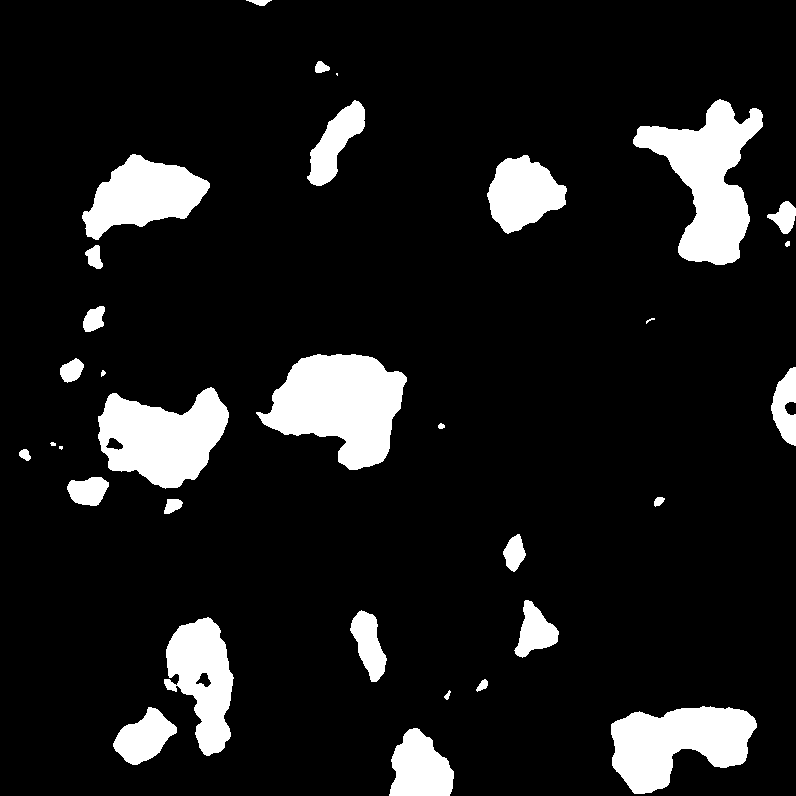
\includegraphics[width=2.0in]{images/ex-simplex-threshold.png}
}

Reexamining the sample texture provided, the shards seem to have more jagged
edges, generally along some lateral axis assuming the shards were rotated. To
obtain this edge behaviour, a parameter was added to the noise to allow for
higher octaves to be stretched in the $x$ direction. On top of this, the noise
function was globally biased towards the x direction, to further compress the
variation in the shard edges along the y axis. This was effective in
adding sharper features and more interested silhouettes. \\

\adjustbox{center} {
    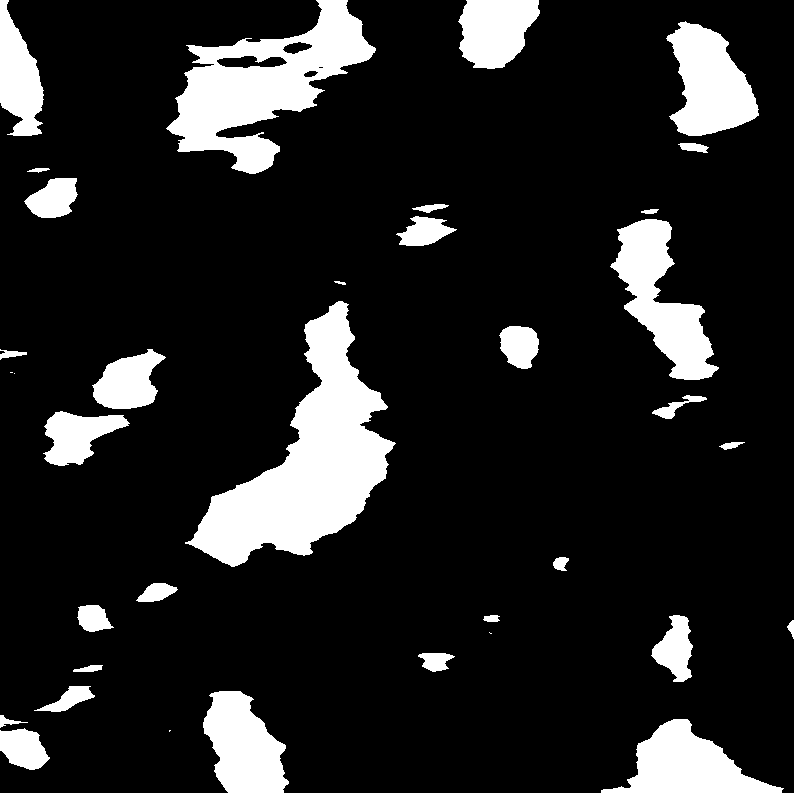
\includegraphics[width=2.0in]{images/ex-simplex-peaks.png}
}
\subsection{Shard Texturing}
At a high level, the provided sample shows a few kinds of local texture applied to each
shard. Large cracks travel across the shards again in their local lateral
directions, aligned with smaller crack-like details aligned in their general
direction. Finally a few small imperfections seem to travel relatively
perpendicular to the main crack directions. 

To generate the large crack texture, the same noise function was used with an extreme
bias towards sampling large intervals in the y coordinate, resulting in the
noise appearing compressed along the height of the image. Also the inverted absolute
value of the noise function was taken to further create sharp peaks. \\

\adjustbox{center} {
    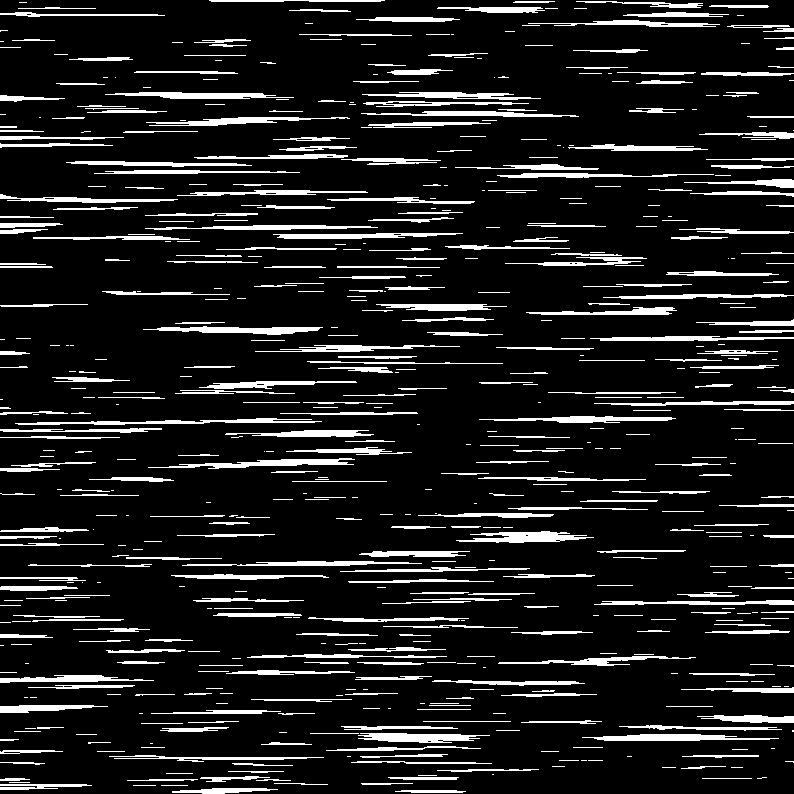
\includegraphics[width=2.0in]{images/large-crack-texture.png}
}

A similar process was used to create the fine surface cracks. The parameters
were tuned to increase the sampling intervals in both directions to generate
higher frequency noise along the same direction as the large cracks.
Additionally, a non-binary cutoff threshold was applied to create more negative
space while still maintaining variation in intensity across the small scratches.

\adjustbox{center} {
    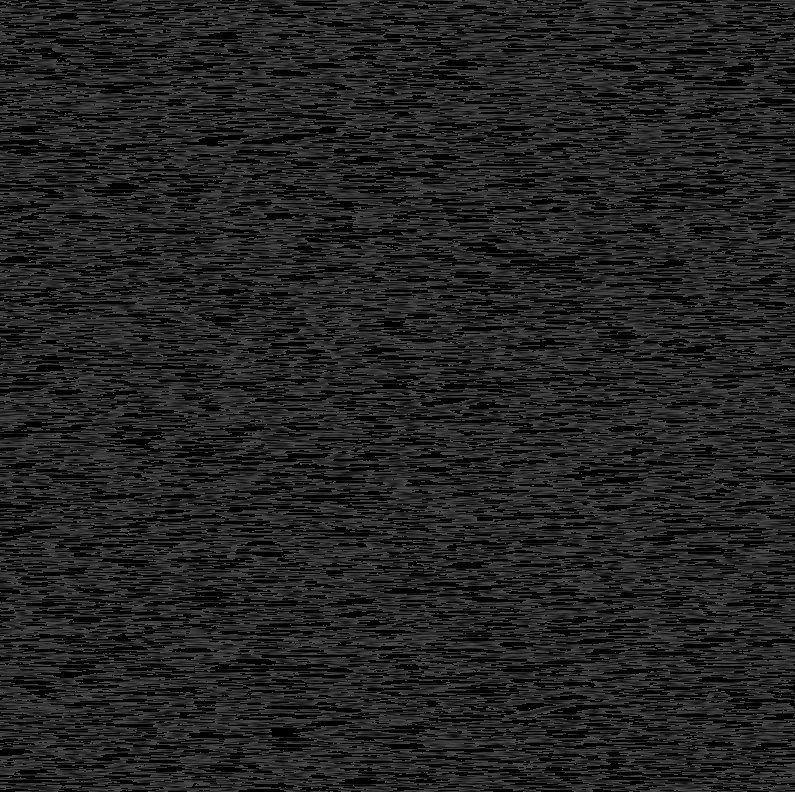
\includegraphics[width=2.0in]{images/small-crack-texture.png}
}

Finally a final set of medium-scale cracks were generated with the opposite coordinate sampling
biases, creating a similar scratch-like pattern but traveling perpendicular to
the main features. To provide more variation, the pattern was rotated by a
random angle.\\

\adjustbox{center} {
    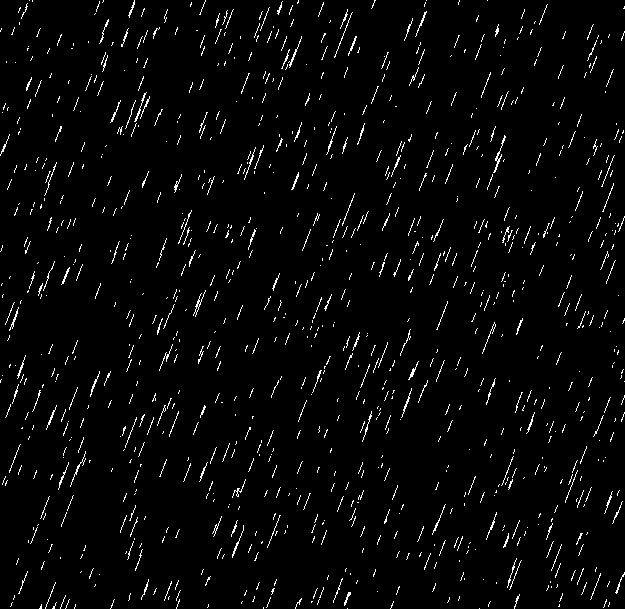
\includegraphics[width=2.0in]{images/cross-cracks.png}
}

Using the initial thresholded shard silhouettes as a mask, the textures were blended overtop
the current shard layer. Adding a base color and blending the surface cracks
with various alpha levels creates the following textured shards.

\adjustbox{center} {
    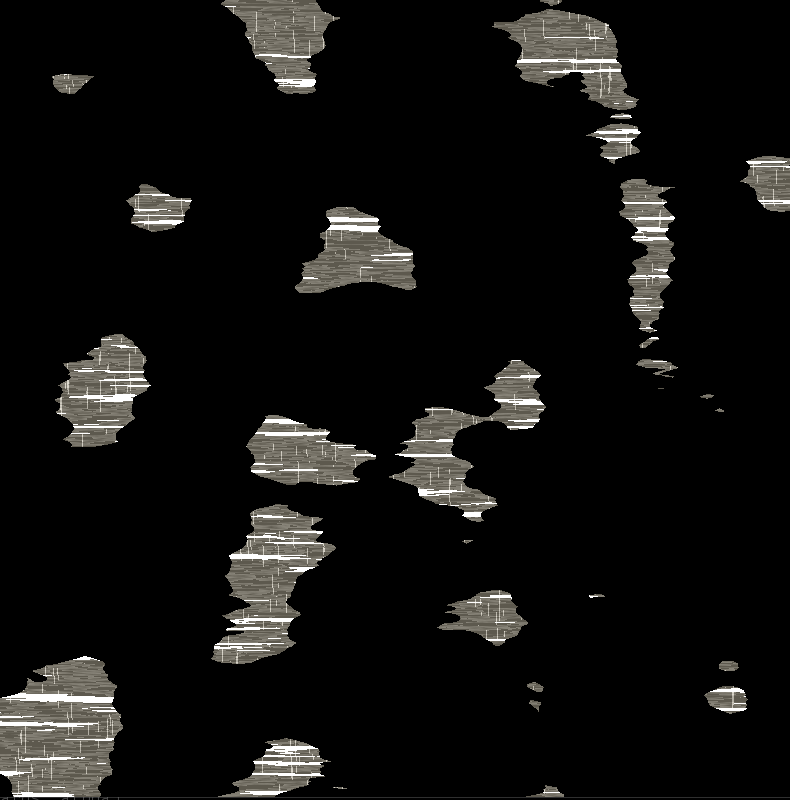
\includegraphics[width=2.0in]{images/textured-shards.png}
}

\subsection{Edge Jittering}
On the original image, the edges of the shards seem to have some light-colored
borders in some areas, likely caused by chips from their formation. To locate
the edges of the shards, a Sobel gradient convolution was applied to the shard
silhouettes and then encoded into an image where the red channel stored the
gradient in the x direction and the blue component stored the y gradient. The
Sobel kernels
\[
\textit{sobel}_x =
\begin{bmatrix}
-1 & 0 & 1 \\
-2 & 0 & 2 \\
-1 & 0 & 1
\end{bmatrix}
\]

\[
\textit{sobel}_y =
\begin{bmatrix}
-1 & -2 & -1 \\
0 & 0 & 0 \\
1 & 2 & 1
\end{bmatrix}
\]

compute the gradient in the x and y directions respectively for a given center
pixel once convolved with an image. The resulting gradient texture shows the
output of the convolution

\adjustbox{center} {
    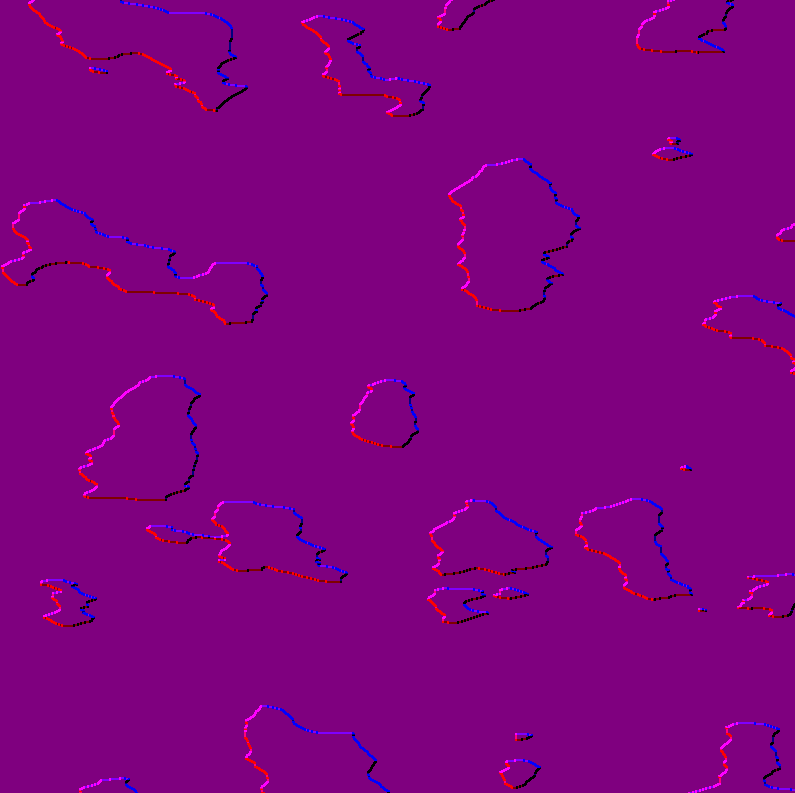
\includegraphics[width=2.0in]{images/shard-gradients.png}
}

To add texture to the edges of the shards, 1 dimensional simplex noise was added
in the direction of dark to light indicated by the gradient mask. This was done
to ensure that the silhouettes of the shards were not effected and instead, the
inner border was textured.  Similarly to
the cracks, the inverse absolute value of the noise was used to create ridges. This resulted in the following mask texture

\adjustbox{center} {
    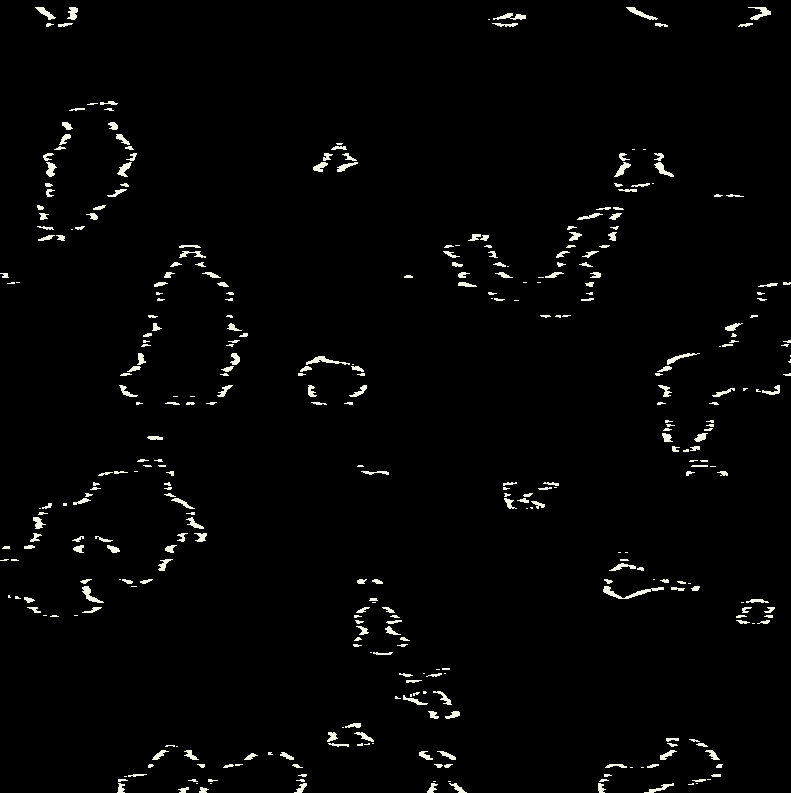
\includegraphics[width=2.0in]{images/jittered-shard-edges.png}
}

Once blended with the previously textured shards, a single final shard layer was
generated.

\adjustbox{center} {
    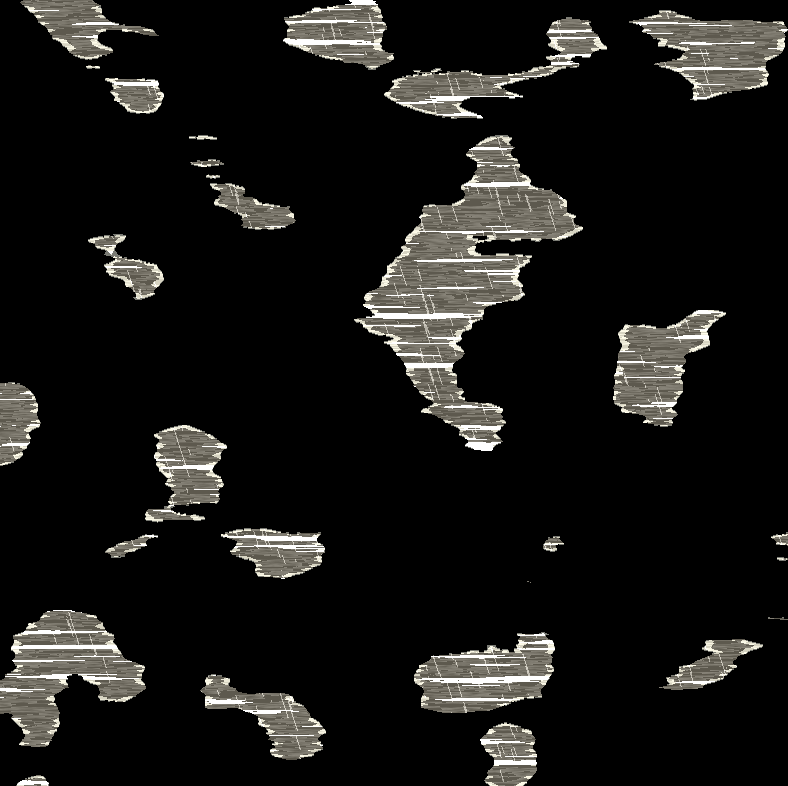
\includegraphics[width=2.0in]{images/textured-shards-with-edges.png}
}

\subsection{Layering}
To obtain the depth of the original image, several of these shard layers were
combined and blended with increasing alpha. A relatively high number of layers
is ideal for creating the illusion of depth and many variations in intensity
between sharps of different layers. Although the local structures examined so
far have focused on the anisotropic lateral features of the shards, in the
original image the shards were placed in various orientations. To achieve this,
each layer is rotated by some random angle in the range [$-\pi/4, \pi/4$].
Naive layering results in a texture similar to an early prototype image shown
below.

\adjustbox{center} {
    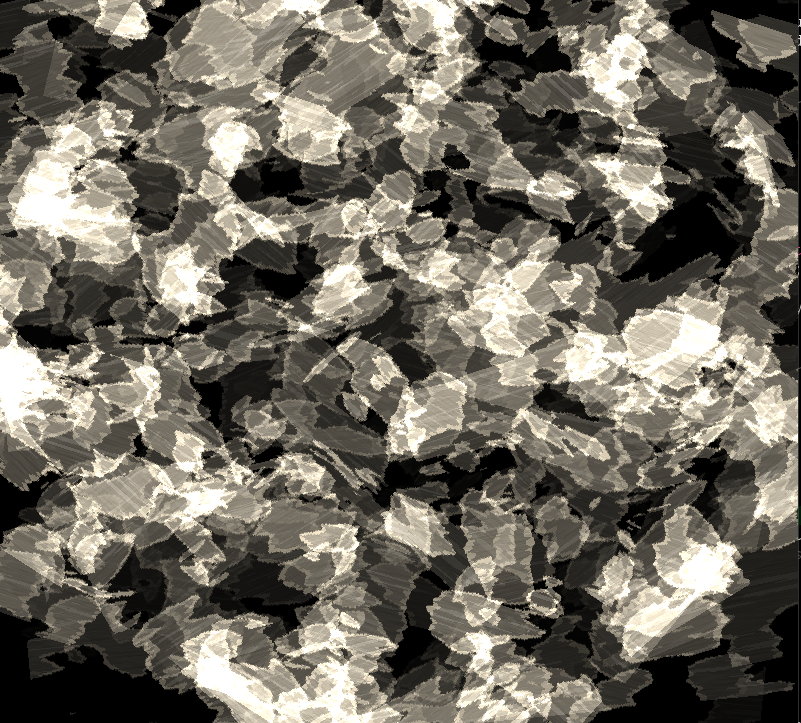
\includegraphics[width=2.0in]{images/spiky shards.png}
}

Although on the right track, the blending often results in patches of extremely
high intensity brightness due to the excessive overdraw. Instead, we want to
layer the only a few shards overtop each other in most areas, avoiding
overblowing the regions towards white. To achieve this, at each layer we invert
the image and use the currently existing empty space as a mask for blending the
new layer onto. Instead of masking only areas that are pure white, we use a mask
intensity that allows us to draw overtop of regions of low to medium intensity
while not pushing the colors to white.

\adjustbox{center} {
    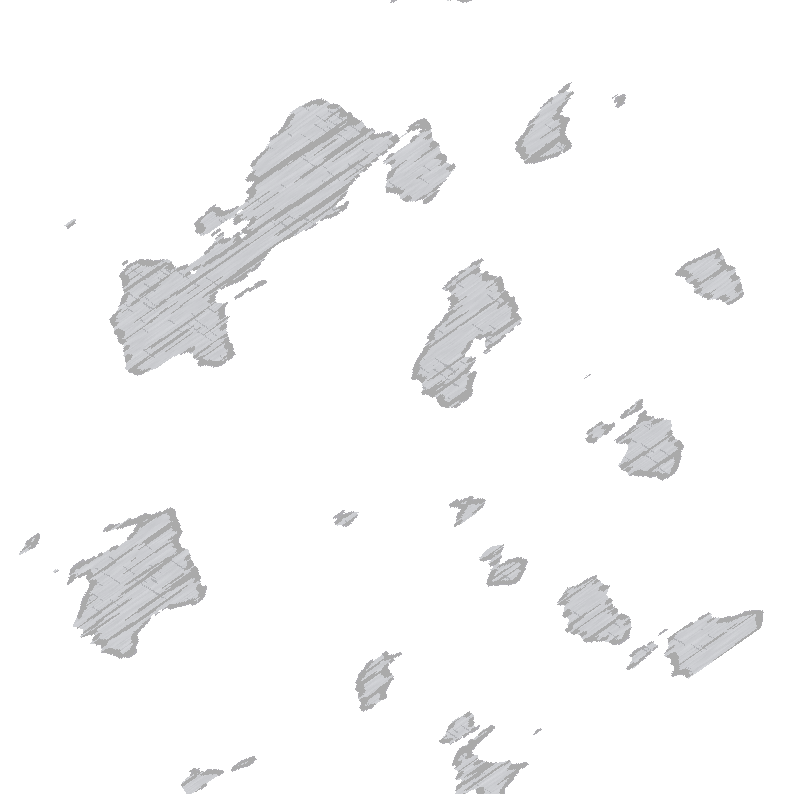
\includegraphics[width=2.0in]{images/masked-shard-layer.png}
}

After applying this progressive layer mask technique, we are left with the following final shard
hierarchy after 20 layers.

\adjustbox{center} {
    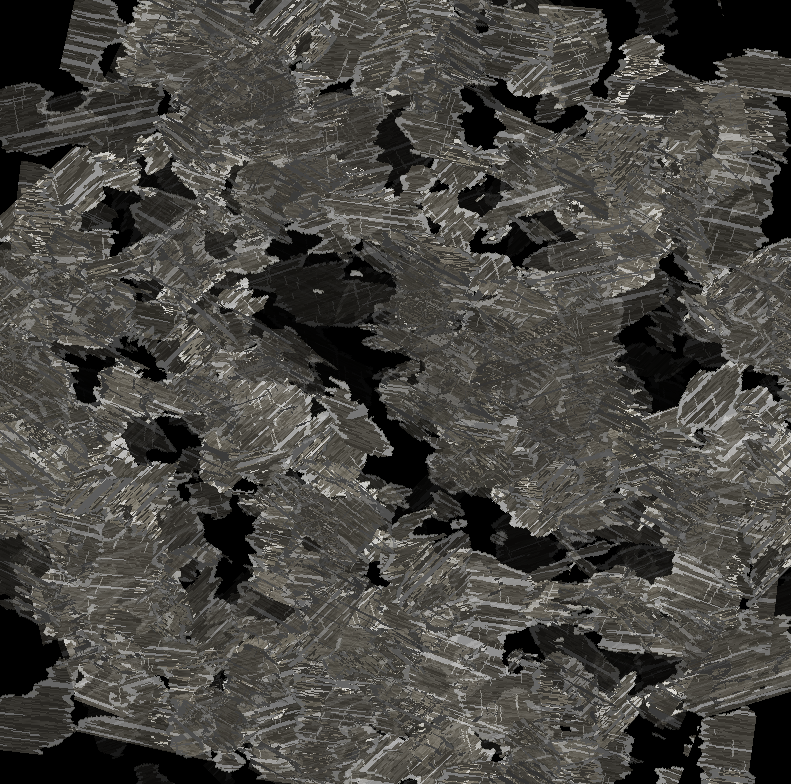
\includegraphics[width=2.0in]{images/no-background.png}
}

Although this masking technique creates some artifacts in the middle of shards
as the mask threshold is in contention with previous layers, these fortunately
create some interesting texture and actually mimic the surface of the shards on
the original image quite well.
\subsection{Background}

To create the cloudy background with small specular pieces, more octave simplex
noise was used. Each octave was given even weighting in the summation, creating
higher frequency noise and variance among regions. A cutoff was placed to create
areas of pure black where the noise value is low. Higher frequency simplex noise
was then used, quantizing the values at two thresholds. One for very bright
specular spots and a second for medium intensity spots. The combined background
looks as follows

\adjustbox{center} {
    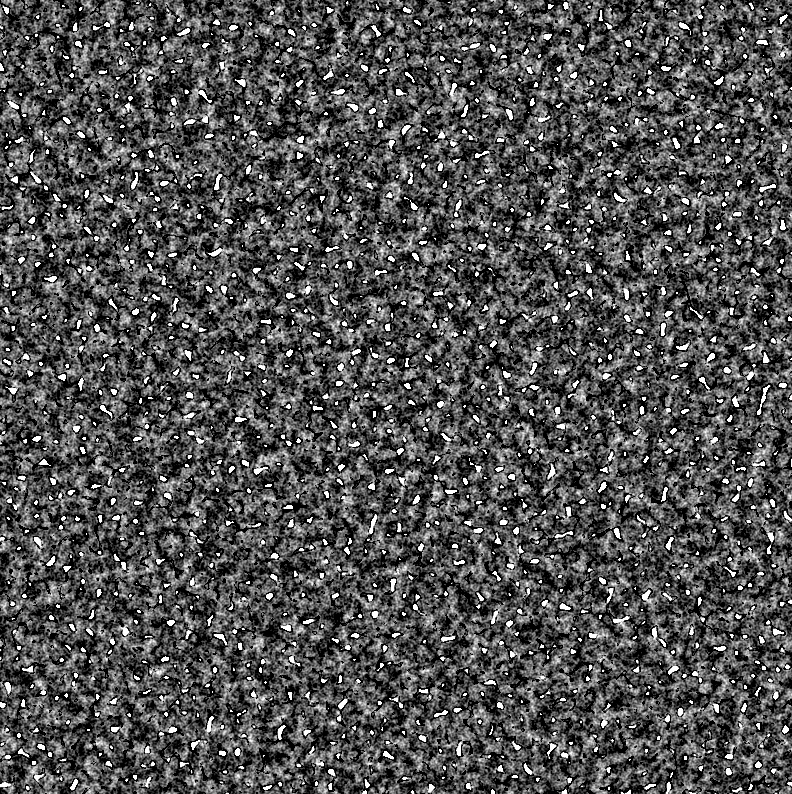
\includegraphics[width=2.0in]{images/background.png}
}

\section{Results}
Combining all stages, here is a sample of a final generated texture along with
the original image

\adjustbox{center} {
    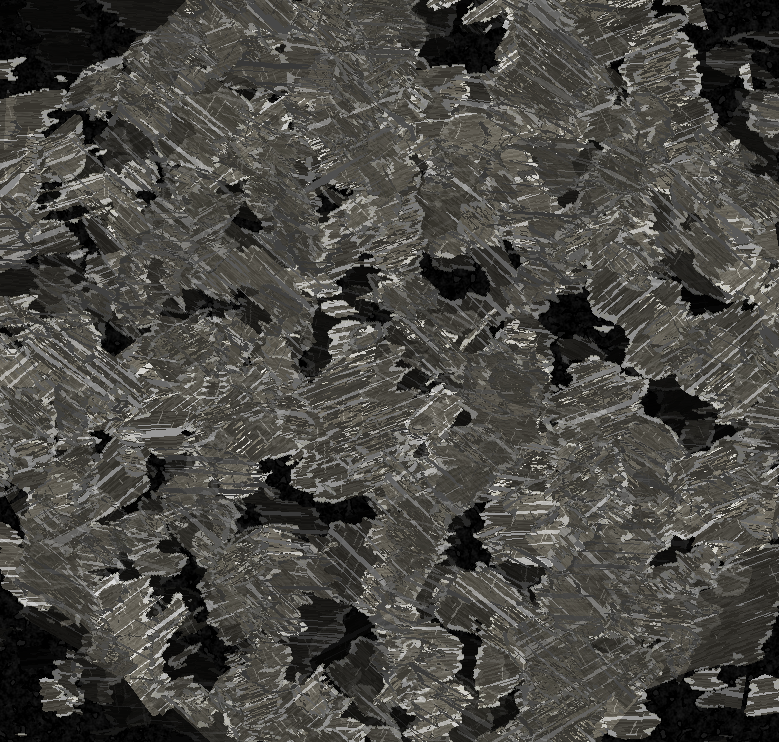
\includegraphics[width=2.0in]{images/final.png}
    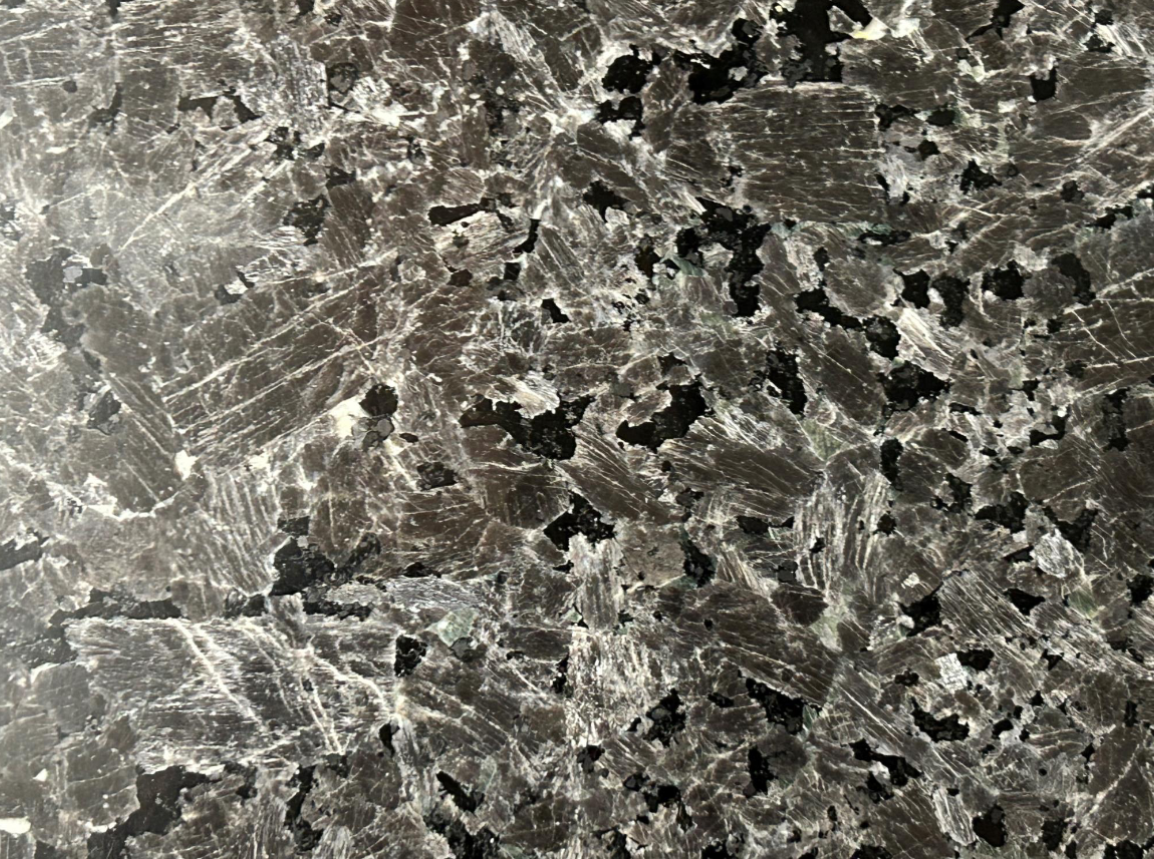
\includegraphics[height=2.0in]{images/sample.png}
}

For a first attempt, the final result in my eyes is good enough at approximating
the general shapes of the granite shards as well as the overall surface texture when
seen at a distance. The shape of the negative space regions between the shards
seems to mirror the sample image extremely closely so I believe the shard
generation strategy is quite sound. However, the generated image lacks the stark
contrast between the shards base color and the cracks that the original has.
Some part of this is likely due to the lack of lighting material properties that
would allow the cracks to reflect light when under similar conditions as the
photo (assuming a high intensity flash). The image rotation also introduces some
discontinuities at the corners which could be ameliorated by more careful
texture sizing and cropping during the generation procedure. In general, my
texture lacks a photo-realistic quality and looks cartoon-like, again likely due
to the simplistic crack textures. Future work should start with improving
contrast along the surface imperfections, doing a more elaborate mask shard
layering, and generating PBR material property textures rather than solely albedo.
\end{document}